% %% Support sites:
%% http://www.michaelshell.org/tex/ieeetran/
%% http://www.ctan.org/tex-archive/macros/latex/contrib/IEEEtran/
%
\documentclass{llncs}
%\documentclass[conference]{IEEEtran}
\usepackage{amsmath,amssymb,amsfonts}
\usepackage{theorem}
%\usepackage{times,mathptm}
\usepackage{times,mathptm}

% *** CITATION PACKAGES ***
\usepackage{cite}

% *** GRAPHICS RELATED PACKAGES ***
\usepackage[dvips]{graphicx}
\graphicspath{{figures/}}
\DeclareGraphicsExtensions{.eps}

% *** MATH PACKAGES ***
%
%%% additional font formatting capability
\usepackage{ulem}
\newcommand{\msout}[1]{\text{\sout{\ensuremath{#1}}}}
%\usepackage[cmex10]{amsmath}
%
\usepackage{algorithm}
\usepackage[noend]{algpseudocode}
\makeatletter
\def\BState{\State\hskip-\ALG@thistlm}
\makeatother
\renewcommand{\algorithmiccomment}[1]{\hfill \footnotesize//~#1\normalsize}

% *** PACKAGE FOR USING THE MULTI-LINE COMMENT ***
\usepackage{verbatim}
\usepackage{color}

% *** ALIGNMENT PACKAGES ***
%
\usepackage{array}
\usepackage{tabularx,ragged2e,booktabs}

% *** SUBFIGURE PACKAGES ***
%\usepackage[font={small}]{caption, subfig}
\usepackage[font=footnotesize]{caption, subfig}

% *** FLOAT PACKAGES ***
%
\usepackage{stfloats}

%% Package to linebreak URLs in a sane manner.
\usepackage{url}
\makeatletter
\def\url@smallurlstyle{%
  \@ifundefined{selectfont}{\def\UrlFont{\sf}}{\def\UrlFont{\small\ttfamily}}}
\makeatother
\urlstyle{smallurl}
\makeatletter
\def\url@tinyurlstyle{%
  \@ifundefined{selectfont}{\def\UrlFont{\sf}}{\def\UrlFont{\scriptsize\ttfamily}}}
\makeatother
\renewcommand{\UrlFont}{\scriptsize}
%
%% Make URLs clickable
\usepackage[colorlinks, bookmarks=false]{hyperref}
%\usepackage{hyperref}
\usepackage{breakurl}
\hypersetup{ colorlinks=false, citecolor=black,
    filecolor=black, linkcolor=black, urlcolor=black
}

%
\usepackage[margin=false,inline=false,marginclue,draft]{fixme}
% REMOVE draft to disable fixme notes
%\usepackage[margin,inline,marginclue]{fixme}
%
\makeatletter
\renewcommand*\FXLayoutInline[3]{%
  {\@fxuseface{inline}\ignorespaces[#3 \fxnotename{#1}: #2]}}
\makeatother

%
% paper title
% can use linebreaks \\ within to get better formatting as desired
\title{Grammar-driven anomaly discovery \\ in time series}

\begin{document} 
\author{Pavel Senin\inst{1} \and Jessica Lin \inst{2} \and Xing Wang \inst{2} \and \\Arnold P. Boedihardjo\inst{3} \and Tim Oates\inst{4} \and \\ Crystal Chen\inst{3} \and Susan Frankenstein\inst{3} \and Sunil Gandhi\inst{4}}

\institute{University of Hawaii, Manoa,
 Dept. of Computer Science, \\
 \email{senin@hawaii.edu}
 \and George Mason University,
 Dept. of Computer Science, \\
 \email{\{jessica , xwang24\} @gmu.edu}
 \and
 U.S. Army Corps of Engineers,
 Engineer Research and  Development Center,
 \email{\{arnold.p.boedihardjo, crystal.chen, susan.frankenstein\}@usace.army.mil}
 \and
 University of Maryland, Baltimore County,
 Dept. of Computer Science,
 \email{oates@cs.umbc.edu, sunilga1@umbc.edu}
}
\maketitle

\begin{abstract}
The problem of anomaly detection in time series has recently received much attention. 
However, many of the proposed techniques require the user to provide the length of the potential anomaly, which is often unreasonable for real-world problems. 
Addressing this limitation, we propose a technique that uses grammar induction to aid anomaly detection without any prior knowledge.  
Our algorithm is capable of discovering co-occurring anomalies of variable lengths, effectively extending the current state of the art.
In addition, we describe a highly efficient variant of our algorithm that is capable of discovering anomalous subsequences of variable length without computing costly distance functions - a procedure that typically accounts for up to 99\% of most algorithms' computation time. 
Finally, we provide an implementation and a visualization tool.


\keywords{time series mining, anomaly discovery}
\end{abstract}


\section{Introduction}
The ability to detect anomalies in time series efficiently is important in a variety of application domains where anomalies convey critical and actionable information, such as in health care, equipment safety, security surveillance, and fraud detection. Consequently, the anomaly detection problem has been studied in diverse research areas \cite{outliers_survey}. Despite the problem's simplicity at the abstract level, where an anomaly is defined as a pattern that does not conform to the underlying generative processes, the problem is difficult to solve in its most general form \cite{chan_anomaly}.

Anomalies in time series can be divided into two broad categories based on their nature: point anomalies and structural anomalies. Point anomalies are defined similarly to those in statistics, i.e. outliers, and are singular data points that are significantly different from others \cite{hawkins}. This type of anomaly has been the most studied \cite{chan_anomaly}. In contrast, a structural anomaly is defined as a subsequence whose shape does not conform to the rest of the observed, or expected, patterns \cite{hot_sax, outliers_survey}. Structural anomalies are similar to contextual anomalies defined in \cite{chan_anomaly} as they presume a notion of context that can be induced from the structure of the dataset or specified as a part of the problem formulation.

While both types of anomalies can be discovered by a na\"{\i}ve approach based on an all-to-all comparison, such a solution has quadratic complexity and is simply impractical for real-world applications. A number of techniques have been proposed to combat the algorithm's complexity \cite{outliers_survey, chan_anomaly}; however, many existing anomaly detection approaches suffer from one or more of the following limitations: (i) they examine each data point independently, without considering their sequential dependency; (ii) they work by matching data points or subsequences with known anomalies or pre-defined thresholds, thus requiring explicit formulation of what is anomalous (or normal); (iii) they require the length of a potential anomaly to be specified. While the first two limitations usually apply to point-based techniques, the third limitation is seen in most, if not all, algorithms that detect structural anomalies. 

In this work we focus on the discovery of structural anomalies and address the above limitations by proposing a technique capable of efficiently detecting anomalies of variable lengths. The proposed algorithm relies on the grammar induction procedure which, once applied to a string obtained by symbolic time series discretization with SAX \cite{sax}, builds a hierarchical structure of context-free grammar rules, each of which maps to variable-length subsequences of the input time series. By analysis of the grammar's hierarchical structure, our algorithm efficiently identifies symbols that are rarely used in grammar rules and whose corresponding subsequences we relate to potential anomalies. 

Before describing our algorithm in detail, consider the following motivational example showing the context-free grammar properties used in our approach. Let 
\begin{center}
$S = abcabcabcXXXabcabc$
\end{center}
be the input string (e.g. derived from a time series) under analysis. Table \ref{table:rules} shows a possible context-free grammar that can be derived from $S$:
\begin{table}[h!] 
\vspace{-0.7cm}
\caption{A possible grammar for the input string $S$} 
\vspace{0.2cm}
\centering
\begin{tabularx}{\linewidth}{X X} % centered columns (2 columns) 
\hline
Grammar Rule & Expanded Grammar Rule \\ 
\hline 
R0 $\rightarrow$ R1 R2 XXX R1 & \textcolor{red}{abc abc} \textcolor{cyan}{abc} \textcolor{blue}{XXX} \textcolor{red}{abc abc} \\ 
R1 $\rightarrow$ R2 R2 & \textcolor{red}{abc abc} \\
R2 $\rightarrow$ abc & \textcolor{cyan}{abc} \\
\hline
\end{tabularx} 
\label{table:rules} % is used to refer this table in the text 
\vspace{-0.5cm}
\end{table} 

The grammar rules reveal repeated patterns via the non-terminals $R1$ and $R2$ --- the context-free grammar property used in motif discovery in our previous work \cite{grammarviz}. Since anomaly detection can be viewed as the inverse problem to motif discovery, we argue that symbols that are rarely used in grammar rules can identify a potential anomaly ($XXX$) as well. The intuition is that subsequences of any length that rarely occur in any grammar rules are non-repetitive, thus most likely to be unusual or anomalous.

If we annotate each symbol of the input string $S$ with a number that is the count of the symbol's appearance in the grammar rules excluding the top-level rule $R0$, the input string $S$ becomes the following:
\begin{center}
$S = a_{2}b_{2}c_{2}a_{2}b_{2}c_{2}a_{1}b_{1}c_{1}X_{0}X_{0}X_{0}a_{2}b_{2}c_{2}a_{2}b_{2}c_{2}$
\end{center}

For example, the first three symbols \{$a$, $b$, $c$\} in $S$ all have a count of 2 because they appear in both $R1$ and $R2$, whereas \{$a$, $b$, $c$\} right before $XXX$ only appear in $R2$. According to our intuition, the set of contiguous points that have the lowest counts, i.e. $XXX$,  correspond to an anomaly.

Note that in the above example, we have not used any explicit distance computation between the grammar's symbols or rules. Moreover, note that the time series discretization technique SAX \cite{sax} and the grammar inference algorithm Sequitur \cite{sequitur} that we rely upon, also do not compute any distance (i.e. they do not explicitly measure how far apart objects are). Taking this into account, unlike most anomaly discovery algorithms, this approach does not require any distance computation on the raw time series. Moreover, since grammar rules naturally vary in length, it enables variable-length anomaly discovery. In addition, we discuss how we use this usage count information to accelerate a more accurate, distance-based algorithm.

\section{Background and Related Work}
In this section, we briefly discuss background and related work on anomaly detection, as well as introduce Sequitur -- our choice for the grammar induction algorithm \cite{sequitur}. We begin by defining our data type:

%\subsection{Definitions}

\begin{definition}
\textbf{Time series} $T = t_{1},\dots,t_{m}$ is a set of scalar observations ordered by time.
\end{definition}
%\vspace{-0.5em}
As we focus on the detection of anomalous patterns, which are likely to be local features, we also consider short subsections of time series called subsequences: 
\begin{definition}
\textbf{Subsequence} $C$ of time series $T$ is a contiguous sampling \\$t_{p},\dots,t_{p+n-1}$ of points 
of length $n << m$ where $p$ is an arbitrary position, such that $ 1 \leq p \leq m - n + 1$.
\end{definition}

In most time series anomaly detection algorithms, the length of anomaly needs to be predefined. Typically, a time series anomaly is considered the most distant (outlying) subsequence under some distance measure $Dist(C,M)$. For example, one of the most commonly used distance measures for time series is the Euclidean Distance. 

%\begin{definition}
%\textbf{Distance} is a function defined for two subsequences $C$ and $M$. The function outputs a non-negative value $R$, which is said to be the distance between $C$ and $M$. 
%\end{definition}

When searching for potential anomalies using a distance function, it is important to exclude self matches---subsequences that overlap the subsequence currently being considered. Such self-matches can yield degenerate and unintuitive solutions as discussed in \cite{hot_sax}. For two subsequences $C$ and $M$ we define a non-self match:
\begin{definition}
\textbf{Non-self match}: given a subsequence $C$ of  length $n$ starting at point $p$ of  
time series $T$, the subsequence $M$ beginning at $q$ is a non-self match to $C$ at distance 
$Dist(C,M)$ if $|p-q| \geq n$.
\end{definition}

One of the most effective methods for time series anomaly detection is via discord discovery. The original work that introduced time series discords, HOTSAX \cite{hot_sax}, defines a discord as follows:

\begin{definition}
\textbf{Time Series Discord}: Given a time series $T$, the time series subsequence $C \in T$ is called the discord if it has the largest distance to its nearest non-self match.
\end{definition}

Discords capture the sense of the most unusual subsequence within a time series and, intuitively, are likely to correspond to many possible anomalies in the generative processes -- a property which was confirmed in a recent extensive empirical study by Chandola et al., where they concluded \textit{"..on 19 different publicly available data sets, comparing 9 different techniques time series discord is the best overall technique among all techniques"} \cite{chan_anomaly}. Since discord discovery has been shown to be the state-of-the-art for time series anomaly detection, we will use the original discord discovery algorithm as the basis for comparison. 

Similar to the notion of discord, we consider time series anomalies to be subsequences that are maximally different from the rest of the subsequences. However, since we work with discretized time series, the way we define ``maximally different'' is not the same. In our approach we rely on the hierarchical structure of conext-free grammar, therefore we define anomalies as substrings that are maximally different in the sense of their normal or abnormal use in the grammar. More specifically, we consider the anomaly to be the subsequence of arbitrary length whose corresponding grammar symbol usage in grammar rules is the smallest.  

\subsection{Previous Work on Anomaly Detection}
The brute force solution for the problem of time series anomaly detection, or more specifically, the discovery of a discord of a given length $n$ in time series $T$ of length $m$, needs to consider all possible distances between each subsequence $C$ of length $n$ and all of its non-self matches $M$ ($C,M \in T$). This method has $O(m^{2})$ complexity and is simply untenable for large data sets. 

In order to mitigate this heavy computational requirement, previous work suggests that the subsequence comparisons should be reordered for efficient pruning. For example, the pioneering work on discord discovery suggests a fast heuristic technique called HOTSAX \cite{hot_sax} that is capable of discovering a true discord by first reordering subsequences by their potential degrees of discordance -- those with a higher chance of being discords are examined first. Secondly, for each discord candidate, the algorithm reorders the matches by their estimated similarity to the potential discord. Similarly in \cite{hashing}, the authors use locality sensitive hashing to estimate similarity between shapes with which they can efficiently reorder the search to discover unusual shapes. The authors of \cite{haar_1} and \cite{haar_2} use Haar wavelets and augmented tries to achieve effective pruning of the search space.

While these approaches achieve several orders of magnitude of speed-up over the brute-force algorithm, their common drawback is that they all need the length of a potential discord to be specified as the input,  and they output discords of a fixed length. %They also require discretization parameters to be specified.
In addition, even with pruning, they rely on the distance computation which, as suggested by Keogh et al.  \cite{hot_sax}, accounts for more than 99\% of the run-time of these algorithms.  

An interesting approach to find anomalies in a very large database (terabyte-sized data set) was shown by Yankov et al.\cite{disk}. The authors proposed an algorithm that requires only two scans through the database. However, this method needs an anomaly defining range $r$ as the input. In addition, when used to detect an unusual subsequence within a time series, it also requires the length of the potential discord.

Some researchers introduced approximate solutions that do not require distance computation on the raw time series. VizTree \cite{viztree} is a time series visualization tool that allows for the discovery of both frequent and rare (anomalous) patterns simultaneously. VizTree utilizes a trie structure to decode the frequency of occurrences for all patterns in their discretized form. Similar to that defined in VizTree, Chen et al.\cite{ano_pattern} also consider anomalies to be the most infrequent time series patterns. The authors use support count to compute the anomaly score of each pattern. Although the definition of anomalies by Chen et al. is similar to discords, their technique requires more input parameters such as the precision of the slope $e$, the number of anomalous patterns $k$, or the minimum threshold. In addition, the anomalies discussed in their paper contain only two points. Wei et al. \cite{bitmaps} suggest another method that uses time series bitmaps to measure similarity. 

Note that many of the algorithms mentioned above \cite{hot_sax, viztree, bitmaps, haar_1, haar_2} transform the time series into a set of strings via SAX (Symbolic Aggregate approXimation), a symbolic representation of time series \cite{sax}, in order to utilize highly efficient data structures designed for discrete data (e.g. tries, hashes, and suffix trees). Our algorithm also relies on SAX, which we discuss in the following section.

\subsection{Frequent Pattern Mining with Sequitur}
Our approach is based on Sequitur, a linear time and space algorithm that derives a context-free grammar from a string incrementally \cite{sequitur}. Although simple in design, Sequitur has been shown to be competitive with state of the art compression algorithms even for very large strings. By identifying and exploiting the hidden hierarchical structure based on recurring subsequences in the input string, the algorithm achieves high computational efficiency while maintaining a relatively small memory footprint. 

%Sequitur works by maintaining two properties: digram uniqueness and rule utility \cite{sequitur}. The first property requires that no pair of consecutive symbols (terminals or non-terminals) appear more than once. Sequitur keeps track of all the digrams by using a hash table (i.e. a digram table). As Sequitur reads in the input string, if it sees a digram already exists in the digram table, i.e., it appears somewhere in the sequence already read, Sequitur uses a non-terminal to substitute these digrams, and, if such a rule does not exist, it forms a new grammar rule with the non-terminal on the left hand side. The second property, rule uniqueness, ensures that each grammar rule is used more than once, except for the top-level rule.

Previously in \cite{grammarviz}, we proposed an algorithm for variable-length time series motif discovery that makes full use of the hierarchy in Sequitur's grammar to find recurrent symbols. Through experimental evaluation we showed that the proposed technique is capable of discovering recurrent patterns of unknown lengths. The algorithm's ability to identify variable-length frequent patterns is based on three characteristic mechanisms: the data smoothing capacity of SAX,  numerosity reduction which effectively enables the patterns' variable length, and Sequitur's utility constraint which ensures that all grammar's non-terminals correspond to recurrent patterns, i.e. motifs.

For this study, we rely on the same approach for transformining the input time series into a hierarchical Sequitur grammar, but instead of finding the most frequent grammar symbols, we show that rarely used symbols of Sequitur grammars are likely to correspond to anomalous subsequences.

\section{Our Approach to Grammar-Based Time Series Decomposition}
As shown above, the main limitation of current anomaly discovery techniques is that they depend on the user-defined subsequence length, which is often unknown in advance. Moreover, a number of variable length anomalous subsequences may co-exist in a time series. It is therefore desirable to have an algorithm that is capable of detecting multiple anomalies without defining their lengths in advance.

Here we present two algorithms for variable-length anomaly detection based on grammar induction. Configured only by discretization parameters, our algorithms are capable of efficiently discovering putative anomalous subsequences without any prior knowledge about their length, shape, or minimal occurrence frequency. While the results produced by our algorithms are approximate solutions, it has been shown recently that in many applications, approximate solutions might be sufficient or even preferable due to efficiency \cite{grammarviz}. 


\subsection{Discretization}
As grammar induction algorithms are designed for discrete data, we begin by discretizing a continuous time series with SAX \cite{sax}. SAX performs discretization by dividing \textit{z}-normalized input time series into $w$ equal-sized segments. For each segment, it computes a mean value and maps it to symbols according to a pre-defined set of breakpoints dividing the distribution space into $\alpha$ equiprobable regions, where $\alpha$ is the alphabet size specified by the user. 

For tasks where localized patterns are of the interest, like anomaly detection or motif discovery, SAX is often applied to a set of subsequences that represent local features. This is called subsequence discretization \cite{lin_motifs}, as opposed to whole discretization where SAX is applied to the entire time series.

\textit{\textbf{Subsequence discretization}}. Our algorithm extracts overlapping subsequences by sliding a window of length $n$ across the time series from its beginning to end. Each of the extracted subsequences is discretized individually using SAX. While most SAX-based techniques shuffle or hash SAX strings into some data structure like a trie or hash table, essentially throwing away the ordering information, we argue that the sequential ordering of the SAX strings provides valuable contexual information, and is the key for allowing variable-length pattern discovery. This produces an ordered set of SAX words, which are then concatenated together to form an input string for Sequitur, i.e. each SAX word is an atomic unit, equivalent to a single terminal for Sequitur. Below we show an example of a SAX-transformed sequence, which is the concatenation (delimited by space) of a set of SAX strings. Each SAX string (e.g. $aac$) represents a subsequence of length $n$ extracted by the sliding window from the original time series.

\begin{center} 
$S1 = \textit{aac~ aac~ abc~ abb~ acd~ aac~ aac~ aac~ abc~} \dots$
\end{center}

\textit{\textbf{Numerosity reduction}}. As we have shown in \cite{lin_motifs}, neighboring subsequences extracted with sliding windows are often similar to each other. When combined with the smoothing properties of SAX, this phenomenon persists through the discretization, resulting in a large number of consecutive SAX words that are identical. Later, these yield a large number of trivial matches significantly affecting the heuristic performance. 

To deal with this issue, we employ a numerosity reduction strategy: if in the course of discretization, the same SAX word occurs more than once consecutively, instead of placing every instance into the resulting string, we record only its first occurrence. Therefore, after numerosity reduction, $S1$ becomes:
\begin{center}
 $S1 = \textit{aac}_{1}~ \msout{\textit{aac}}_{2}~ \textit{abc}_{3}~ \textit{abb}_{4}~ \textit{acd}_{5}~ \textit{aac}_{6}~ \msout{\textit{aac}}_{7}~ \msout{\textit{aac}}_{8}~ \textit{abc}_{9}$ \\
 $ = \textit{aac}_{1}~ \textit{abc}_{3}~ \textit{abb}_{4}~ \textit{acd}_{5}~ \textit{aac}_{6}~ \textit{abc}_{9}$ 
\end{center}
where subscripts in the resulting string denote the offsets of the original SAX words occurrences. In addition to speeding up the algorithm and reducing its space requirements, numerosity reduction procedure provides an important feature in this work -- it enables the discovery of variable-length anomalies. 

\subsection{Grammar Induction on SAX Words}\label{rule_utility}
Once we transform a time series into a string of SAX words, we can then apply Sequitur to build a context-free grammar, which essentially is a hierarchical structure that recursively reduces all \textit{digrams} occurring more than once in the input string to a single new non-terminal symbol. This corresponds to the Sequitur-specific ``rule utility'' constraint that we use later for the anomaly discovery. A digram is a consecutive pair of tokens (terminals or non-terminals). As mentioned, we consider a SAX string as an atomic unit (i.e. a terminal). A digram consisting of two terminals is thus a pair of consecutive SAX strings, e.g. \{$aac$ $abc$\}.

To reiterate the benefit of the numerosity reduction strategy mentioned above and how it lends itself to variable length anomalies or motifs, consider the single grammar rule $R1$ generated by Sequitur from the string \textit{S1} as shown in Table \ref{table:rulesS1}:
\begin{table}[h] 
\vspace{-0.8cm}
\caption{A Sequitur grammar for the input string $S1$} 
\vspace{0.2cm}
\centering
\begin{tabularx}{\linewidth}{X X}
\hline
Grammar Rule & Expanded Grammar Rule \\
\hline
$\text{R0}~ \rightarrow~ \text{R1}~ \text{abb}~ \text{acd}~ \text{R1}$ & $ \textcolor{red}{aac}_{1}~ \textcolor{red}{abc}_{3}~ abb_{4}~ acd_{5}~ \textcolor{red}{aac}_{6}~ \textcolor{red}{abc}_{9}$ \\ 
$\text{R1}~ \rightarrow~ \text{aac}~ \text{abc} $ & $\textcolor{red}{aac}~ \textcolor{red}{abc}$ \\


\hline
\end{tabularx}
\label{table:rulesS1} % is used to refer this table in the text 
\vspace{-0.4cm}
\end{table} 

In this grammar, $R1$ concurrently covers intervals of different lengths: $S1_{[1:3]}$ of length 3, and $S1_{[6:9]}$ of length 4 respectively. The potential anomalous substring ``$abb_{4}$ $acd_{5}$'' has length of 2. Recall each SAX string corresponds to a time series subsequence, so these intervals correspond to subsequences of variable lengths. 

\subsection{Using Grammar Rules to Find Anomalies}
By keeping SAX words offsets throughout the procedures of discretization and grammar construction, our algorithm is able to map rules and SAX words back to their original time series subsequences. The number of rules generated by Sequitur can be large. In this work, we rank grammar rules by their ``potential'' of being an anomaly, which, according to our intuition, is proportional to their usage frequency. Further, we discuss two concrete algorithms for variable-length anomaly discovery based on this ranking scheme.

\section{Grammar-Driven Anomaly Discovery}
In the previous section we described a number of successive steps which allow us to represent a time series as a hierarchical structure composed of context-free grammar rules. Here, we present two algorithms for variable-length anomaly discovery that exploit the grammar-based representation. 
The first algorithm is designed for highly efficient discovery of variable length putative anomalies and is solely based on the usage frequency of grammar symbols, i.e. this algorithm does not compute distance between raw subsequences nor strings. While the algorithm is highly efficient and can be used for very large data sets, its effectiveness can be severely affected by improper parameter choices.
The second algorithm also enables efficient discovery of putative anomalies of variable length and is more robust than the discrete parameter choice. This algorithm extends the HOTSAX approach -- the current state of the art for discord discoveries, and relies on  distance computations.

\begin{figure}[t]
   \vspace{-0.2cm}
   \hspace{-0.3cm}  
   \includegraphics[width=122mm]{Figure2_ECG0606.ps}
   \caption{An example of discords discovery in ECG dataset (Physionet QT Database, record 0606 \cite{physionet}). Top panel shows the anomalous heartbeat location. Middle panel shows that the approximate anomaly discovery approach based on Sequitur rule density can clearly identify the true discord -- almost no rules span the anomaly. Bottom panel confirms that the distance-based anomaly discovery technique also finds the true anomaly since the grammar rule that spans the anomaly has the largest distance to its nearest non-trivial match among all other subsequences.}
   \label{fig:ecg}
   \vspace{-0.3cm}
\end{figure}

\subsection{Rule Density-Based Anomaly Discovery}
To discover approximate anomalies efficiently, we propose to compute the ``\textit{rule density}'' curve for the input time series. To do this, an empty array of length $m$ (the time series length), is first created. Each element in this array corresponds to a time series point and is used to keep count of the grammar rules that span (or ``cover'') the point. Second, since the locations of relevant subsequences for all grammar rules are known, by iterating over all grammar rules the algorithm increments a counter for each of the time series points that the rule spans. After this process each element of the array contains a value indicating the total number of grammar rules that cover a corresponding time series point. We call this array the \textit{rule density array} and the corresponding curve the \textit{rule density curve}. As an example, consider the rule density curve shown in the middle panel of Figure \ref{fig:ecg}.

Since each SAX string corresponds to a subsequence starting at some position of the time series, the points whose rule density counters have a globally minimal value thus correspond to the grammar symbols (terminals or non-terminals) whose inclusion in the grammar rules is minimal. Therefore, similar to the discussion for the rules in Table \ref{table:rules}, we argue that the \textit{rule density curve intervals which contain minimal values correspond to time series anomalies}. 

Consider the example shown in Figure \ref{fig:ecg}. The top panel shows an excerpt of an ECG time series with a highlighted instance of an anomalous heartbeat featuring a very subtle premature ventricular contraction. The middle panel shows a significant drop in the grammar rule density in this case corresponding with the global minimum (3 rules) over the interval 462-482, which is in perfect alignment with the ground truth -- the annotation by an expert which states that an anomaly occurs in the ST interval of the ECG curve, located at the rightmost part of the red-colored heartbeat.  

This rule density-based approach is capable of discovering multiple anomalies of variable-length by its design -- it simply reports contiguous points of the input time series which appear to be covered by the globally minimal number (ideally, zero) of grammar rules. If needed, an additional ranking criterion can be defined: for example a minimal anomaly length and/or a minimal coverage threshold or their ratio can be used to tolerate noisy data.

Note, however, that from our experience, this rule density-based technique only approximately indicates an anomaly location and its accuracy largely depends on the choice of SAX discretization parameters (including the initial subsequence length) and ultimately on the data (generative process) specificity. Also note, that even though we need to specify the subsequence length, it is only the initial ``seed.'' Unlike most existing algorithms in which this subsequence length is the exact length of the anomaly, anomalies reported by our technique are not bounded by the seed length and may range from very short to considerably long values.
\enlargethispage{\baselineskip}

Another desirable characteristic of this approach is the efficiency. SAX, the discretization technique, has a linear time complexity \cite{hot_sax} as well as the grammar inference technique, Sequitur \cite{sequitur}. The coverage curve computation itself has a linear complexity too as it involves iteration over the number of grammar rules, which is always less than the input string, and simple counting. This efficiency, when combined with effective visualization (Section \ref{section_implementation}), enables the user to interactively explore the dataset and to refine discretization parameters and the anomaly selection threshold.

\begin{algorithm}[!htp]
\caption{SAXSequitur algorithm (modified HOTSAX)}\label{algorithm2}
\begin{algorithmic}[1]
\Procedure{Heuristic\_search}{$T,n,RuleSubsequences,Outer,Inner$}
 \State $\text{best\_so\_far\_dist} = 0 $
 \State $\text{best\_so\_far\_loc} = \text{NaN} $
 \For{\textbf{each} $p$ in $RuleSubsequences$ ordered by heuristic $Outer$}\Comment{We completely}
 \Statex{}\Comment{change this heuristic}
    \State nearest\_neighbor\_dist = Infinity
    \For{\textbf{each} $q$ in $T$ ordered by heuristic $Inner$}\Comment{We partially change}
    \Statex{}\Comment{this heuristic}
       \If {$| p -– q | \geq n$ } 
           \If { $Dist (t_{p},...,t_{p+n-1}, t_{q},...,t_{q+n-1}) < \text{best\_so\_far\_dist}$ }
               \State {\textbf{break}} 
           \EndIf 
           \If {$Dist (t_{p},...,t_{p+n-1}, t_{q},...,t_{q+n-1}) < \text{nearest\_neighbor\_dist}$ }
               \State $\text{nearest\_neighbor\_dist} = Dist (t_{p},...,t_{p+n-1}, t_{q},...,t_{q+n-1})$
           \EndIf 
       \EndIf 
    \EndFor
 \If {$\text{nearest\_neighbor\_dist} > \text{best\_so\_far\_dist}$} 
   \State $\text{best\_so\_far\_dist} = \text{nearest\_neighbor\_dist}$ 
   \State $\text{best\_so\_far\_loc} = p$
 \EndIf   
 \EndFor
 \State \textbf{return} $(\text{best\_so\_far\_dist}, \text{best\_so\_far\_loc})$
\EndProcedure
\end{algorithmic}
\end{algorithm}

\subsection{Distance-Based Anomaly Discovery}
If the time series under analysis is aperiodic, or the discretization parameters are far from optimal, the rules coverage-based anomaly discovery technique can fail due to the high number of grammar rules covering large spans of the time series, or due to the large number of uncovered subsequences. Moreover, some applications may need an additional anomaly evidence, such as the largest distance to its nearest non-self match. To address this issues, we propose another variant of a grammar-driven variable-length discord discovery algorithm that is based on distance computation and allows more accurate anomaly discoveries. This technique modifies the HOTSAX \cite{hot_sax} algorithm by adding grammar induction to significantly improve the efficiency of the original heuristics. The SAXSequitur algorithm overview is shown at the panel Algorithm \ref{algorithm2}.

As we mentioned before, by efficiently optimizing the search order through heuristics, HOTSAX significantly improves the brute force algorithm performance without sacrificing accuracy. The original algorithm consists of two nested loops that iterate over all possible time series subsequences in optimized order. 

To facilitate fast computational time and allow for variable-length discord discovery, we propose an improvement to the original $Outer$ heuristic by utilizing the information from the grammar structure discovered by Sequitur. More specifically, we analyze the grammar and create an ordered list of subsequences called $RuleSubsequences$ which contains all subsequences for all grammar rules sorted in the ascending order of rule usage frequency. The intuition behind this ordering is simple and is a reflection of previously discussed grammar property suggesting that rarely used grammar rules are likely to correspond to anomalous subsequences. If there exist time series points with zero usage count (i.e. points that are not included in any grammar rules), they need to be added to the $Outer$ list too. 

We also alter the $Inner$ heuristic. First, having a candidate subsequence from a grammar rule selected in the $Outer$ loop, we consider all other subsequences from the same rule as possible nearest non-self matches. After this step, the rest of the subsequences are visited in random order. The intuition behind this ordering is also simple and similar to that of HOTSAX -- the 
candidate subsequences corresponding to the same SAX string, or to the Sequitur rule in our case, are very likely to be highly similar. Thus, considering such subsequences in the beginning of $Inner$ heuristic allows us to potentially encounter a distance that is smaller than $best\_so\_far\_dist$ sooner and to benefit from the early abandoning (lines 8 and 9 of the Algorithm \ref{algorithm2}) while considering all other candidates in $Outer$ loop. Note that since the subsequences are of variable lengths, we cannot use the Euclidean distance directly on the subsequences. There are two potential approaches: (1) reinterpolate the subsequences to equal length and use Euclidean distance; and (2) use an elastic distance measure such as Dynamic Time Warping (DTW), and normalize the distance for meaningful comparison. For the current study, we opted for option 1, but we plan to investigate the potential of option 2 for future work. 

\begin{figure}[!t]
   \vspace{-0.3cm}
   \centering
   \includegraphics[width=120mm]{DutchPD_new.ps}
   \caption{An example of the multiple discord discoveries in Dutch power demand data set with SAXSequitur. Top panel shows the data set overview - 52 weeks of power demand by a research facility. Middle panel shows that while the approximate discord discovery technique was able to discover the best discords (colored red), next two anomalies are difficult to quantify. Bottom panel shows that the exact discord discovery technique is able to discover and to rank all discords.}
   \label{fig:dutch_PD}
   \vspace{-0.3cm}
\end{figure}

Our new SAXSequitur heuristic allows us to discover subsequences of variable length. Note, however, that in contrast to HOTSAX our algorithm does not guarantee the discovery of the best discord since it does not consider all possible candidate subsequences in the $Outer$ loop due to their variable lengths.

Examples of discords found are shown in the bottom panels of Figures \ref{fig:ecg} and \ref{fig:dutch_PD}, where we indicate locations and true distances from each time series subsequence corresponding to a Sequitur rule and their nearest non-self match by a vertical line placed at the rule beginning and whose height equals the distance. Clearly, the rules which partially overlap with the anomalous heartbeat, or the anomalous weekly energy demand have the most distant nearest neighbor. Our algorithm is also capable of outputting a list of multiple co-existing discords of variable length, as shown in Figure \ref{fig:dutch_PD2}. Better-quality images and more results can be found on \url{http://www.cs.gmu.edu/~jessica/GrammarDiscord.html}.

\begin{figure}[!t]
 \vspace{-0.3cm}
 \centering
 \includegraphics[width=120mm]{DutchPD_new1.eps}
 \caption{A detailed view of power demand by a Dutch research facility during an average week along with three anomalous locations discovered by SAXSequitur. Note all three discords are of slightly different lengths.}
 \label{fig:dutch_PD2}
 \vspace{-0.3cm}
\end{figure}

\begin{figure}[t]
   \vspace{-0.2cm}
   \hspace{-0.1cm}  
   \centering
   \includegraphics[width=123mm]{ECG2_screen_density.eps}
   \caption{
   SAXSequitur rule density display aiding in visual anomaly discovery. The background color intensity value corresponds to the density of Sequitur rules. Note the low background color intensity between positions 400 and 500 where an anomalous heartbeat is located.}
   \label{fig:densityECG}
   \vspace{-0.3cm}
\end{figure}

\section{Our Implementation: SAXSequitur}\label{section_implementation}
Depending on the complexity of the dataset and choice of SAX parameters, the number of rules generated by Sequitur can be large. Moreover, since the proposed algorithms' performance depends on the discretization parameters, it is highly desirable to have an exploratory tool that not only allows the user to visually navigate and examine found patterns and anomalies, but also provides a means for interactive parameter tuning.

Addressing this issue, we extended our previous grammar/motif visualization prototype with an implementation of the proposed methodology. We call our system \textit{SAXSequitur}. Our stand-alone GUI application implements all steps of the proposed approach enabling visual data exploration, interactive discretization and numerosity reduction parameter tuning, and visualization of the grammar rules along with their corresponding motif and discord patterns. SAXSequitur is implemented in Java and is a cross-platform application designed following the Model-View-Controller (MVC) pattern, offering further extensibility. Its source code is publicly available at \cite{jmotif}.

The user interface of our tool consists of a number of panels where the largest is the \textit{Data display} which provides an overview of the dataset under analysis. Right below, the second largest panel, presents Sequitur rules through two interface widgets: an interactive table of \textit{Sequitur rules} that provides rule statics and a \textit{Rule Subsequence Display} window that shows all subsequences corresponding to a selected rule. Other panels allow users to select and load a new dataset (\textit{Data source} panel), tune the discretization strategy, SAX parameters, and choose the numerosity reduction strategy (\textit{SAX parameters} panel). The bottom panel provides a system log. Figure \ref{fig:densityECG} shows an example of the rule density visualization for the ECG dataset discussed above.
Our visualization approach is based on transforming the time series into the user-configured symbolic representation, building a grammar with Sequitur, and mapping the grammar rules back to the time series. After performing these steps, SAXSequitur creates a single data structure which is used in the interactive visualization. The rule statistics includes the frequency of rule's  use by other rules, the rule itself and its expanded form, frequency of occurrence, average length, and positions at which it occurs in the SAX string and in the time series; the rules table is fully interactive. 

\section{Experimental Evaluation}
We evaluated both proposed techniques (Rule-density-based and SAXSequitur heuristic) on a number of previously studied data sets and compared their performance with both: the brute force and HOTSAX (current state of the art \cite{chan_anomaly}) discords discovery algorithms. 

As expected, discords discovered by HOTSAX matched those of brute force exactly. However, since our technique optimizes candidate anomaly selection by using Sequitur grammar structure, the locations of anomalies discovered by SAXSequitur were not exactly the same, but in close neighborhood of the true discords. In addition, we found that more stringent parameters were needed to achieve a significant overlap of discovered anomalies by the distance-based SAXSequitur algorithm. Note, that by increasing SAX discretization granularity we effectively limit the variability of rule lengths, thus, we effectively approximate HOTSAX algorithm behavior. 

The SAXSequitur heuristic algorithm was also able to discover known anomalies in \textbf{all} data sets, though, more careful parameters selection were at times needed. However, we found that the rule density-based technique allows the discovery of very short anomalies that the three other techniques missed. For example, in the GPS trail dataset the rule density-based technique was the only method capable of discovering a true anomaly which was intentionally planted by taking an unusual path.

Finally, we compared algorithms performance in terms of calls to the distance computation routine, which, as pointed in \cite{hot_sax} typically accounts for up to 99\% of
these algorithms computation time. Table \ref{perf_table} compares the number of distance function calls made by the competing techniques. 

\begin{footnotesize}
\begin{table}[t]
\vspace{-0.2cm}
\caption{Performance comparison of anomaly discovery algorithms.}
\label{perf_table}
\centering
\begin{tabularx}{\linewidth}{X r r r r r }
\hline
 Dataset & Length & & \multicolumn{3}{c}{Number of calls to distance function}\\ 
 \cline{4-6}
 &  & & Brute-force & \textit{HOTSAX}
& SAXSeqitur \\
\hline
\raggedright
Daily commute GPS track & 17'175 & & 271'376'202 & 879'067 & 112'405 \\
Dutch research facility power demand & 35'040 && $1.13 \times 10^{9}$ & 6'196'356 & 327'950\\
ECG 0606 & 2'300 & & 4'399'506 & 72'390 & 16'717 \\
ECG 308 & 5'400 & & 23'025'602 & 327'454 & 14'655 \\
ECG 100 & 5'401 & & 23'035'200 & 1'206'684 & 29'599 \\
ECG 15 & 15'000 & & 218'995'602 & 1'434'665 & 111'348 \\
ECG 108 & 21'600 & & 416'098'802 & 6'041'145 & 150'184 \\
ECG 300 & 536'976 & & $288 \times 10^{9}$ & 178'428'955 & 9'195'453 \\
ECG 318 & 586'086 & & $343 \times 10^{9}$ & 32'786'225 & 3'395'177 \\
TEK14 & 5'000 & & 22'491'306 & 691'194 & 48'226 \\
TEK16 & 5'000 & & 22'491'306 & 61'682 & 15'573 \\
TEK17 & 5'000 & & 22'491'306 & 164'225 & 78'211 \\
\hline
\end{tabularx}
   \vspace{-0.5cm}
\end{table}
\end{footnotesize}

In short, rule-density-based approach, when used alone, is fast since it does not require any distance computation, but it fails to find some subtle discords. Incorporating rule density into the HOTSAX framework (i.e. the SAXSequitur heuristic), however, enables us to discover discords in all data sets. It's faster than HOTSAX and brute-force, and it allows the discovery of variable-length discords. 

\subsection{Parameter Setting}
Like all SAX-based algorithms, we need to set two parameters: the number of PAA segment ($w$) and the alphabet size ($\alpha$). In addition, we need to set the initial subsequence length (the ``seed'' that will grow with grammar induction). The choice of initial length is not as critical as most existing anomaly detection algorithms, where the input length is the exact length of the anomaly. In our experiments, we try various initial length values (100-300), number of PAA segments (mostly 4 or 6, in some cases higher values), and alphabet size (4-6). The rule-density approach alone is more sensitive to the parameter choices than if it's incorporated in the SAXSequitur heuristic. Nevertheless, the rule density approach still offers the advantage of providing fast discord approximation. 

\subsection{Spatial Trajectory Case Study}
To demonstrate the application and effectiveness of SAXSequitur for discovering anomalies of unknown nature, we performed a case study on spatial trajectory data. The data was gathered from a GPS device which recorded location coordinates and times at certain temporal intervals while commuting. To apply SAXSequitur to the trajectory data, the trajectory data (lat, lon) was transformed into a sequence of scalars. To achieve this, the trajectory points are mapped to the visit order of a Hilbert space filling curve (SFC) embedded in the trajectory manifold space and indexing the recorded times of the visit order. The Hilbert SFC is chosen to reduce the distortion on the data's spatial locality. The sequence of SFC visit order along with their times is passed to the SAXSequitur algorithm for processing. 

In the GPS data, multiple trajectories representing daily commute are recorded for an individual. Generically, a trajectory anomaly is defined as a sub-trajectory path that is atypical in the set of paths taken by an individual. Specifically, an anomaly can either be a sub-trajectory that occurs in rarely visited spatial regions such as a detour, or a novel path taken within a frequently visited spatial region. The second type of trajectory anomaly is important because it considers the order by which the various locations are visited. For instance, if multiple points in a space are visited frequently, the occurrence of a visit to these points is not an anomaly; however, the occurrence of visiting these points in an unseen order is an anomaly. 

In order to evaluate the proposed algorithm efficiency on this specific data, we intentionally introduced a few anomalies by taking atypical turns and routes and travelling on bicycle on bike routes which are close to the city roads. Figures \ref{fig:gps} and \ref{fig:gps2} show the results of the discovered anomalies in the GPS tracks. In Figure \ref{fig:gps}, both algorithms were able to successfully detect the anomalies: low frequency path and signal loss event. Figure \ref{fig:gps2} highlights SAXSequitur's ability to capture the more difficult anomaly, unexpected path within highly visited spatial regions. These results show promise that our proposed algorithms are able to discover significant anomalies in trajectory data. 

\begin{figure}[t]
   \centering
   \vspace{-0.5cm}
   \includegraphics[width=120mm]{path_figure.eps}
   \caption{An example of grammar-driven anomaly discovery in the transformed with Hilbert SFC GPS track. The best discord (red colored) was discovered by both algorithms and corresponds to a track segment that was travelled only once. While the second discord indicates the track segment where some GPS signal loss occurred.}
   \label{fig:gps}
   \vspace{-0.35cm}   
\end{figure}

\section{Conclusions and Future Work}
In this work we introduced two novel algorithms for anomaly detection in time series based on grammar induction. We show that by exploiting the hierarchical structure of context-free grammar, it is possible to discover anomalous subsequences in a highly efficient way. In addition to being comparable in accuracy with the current state of the art, our algorithms demonstrate superior efficiency and are also capable of finding variable length anomalies. Furthermore, we implemented a visualization software based on the techniques proposed, that provides a highly interactive and exploratory pattern mining environment. For future research, we plan to investigate the effect of more sophisticated distance measures, such as DTW, on the algorithm performance. In addition, we would like to perform a study on the algorithms' sensitivity to parameter selection.  

\begin{figure}[t]
   \centering
   \vspace{-0.5cm}   
   \includegraphics[width=122mm]{gps_zoom.eps}
   \caption{An example of anomalies discovered in GPS track by SAXSequitur. Left panel shows the anomalous track which does not conform to the typical behavior of exiting from and entering the block. The right panel shows the anomalous track segment that contains an interval traveled without GPS fix.}
   \label{fig:gps2}
   \vspace{-0.35cm}   
\end{figure}


\begin{thebibliography}{4}

%1
\bibitem {outliers_survey}
Gupta, M., Gao, J., Aggarwal, C.C., Han, J.:
Outlier Detection for Temporal Data: A Survey.
IEEE Trans. on Knowledge and Data Engineering, 25, 1, (2013)

%2
\bibitem{chan_anomaly} Chandola, V., Cheboli, D., and Kumar, V.:
Detecting Anomalies in a Time Series Database.
CS Technical Report 09--004, (2009)

%3
\bibitem{hawkins} Hawkins, D. M.: 
Identification of Outliers. Chapman and Hall, (1980)

%4
\bibitem {hot_sax}
Keogh, E., Lin, J., Fu, A.:
HOT SAX: Efficiently Finding the Most Unusual Time Series Subsequence. 
In Proc. ICDM. 226--233, (2005)

%5
\bibitem {sax}
Patel, P., Keogh, E.,, Lin, J., Lonardi, S.:
Mining Motifs in Massive Time Series Databases. 
In Proc. ICDM, (2002)

%6
\bibitem{grammarviz}
Y. Li, J. Lin, and T. Oates. 
Visualizing variable-length time series motifs. 
In Proc. of the 2012 SIAM International Conference on Data Mining, 895-906, (2012)

%7
\bibitem {sequitur}
C.G. Nevill-Manning and I.H. Witten.:
Identifying Hierarchical Structure in Sequences: A linear-time algorithm. 
Journal of Artificial Intelligence Research, 7, 67-82, (1997)

%8
\bibitem{hashing} 
Wei, L., Keogh, E., Xi, X.: 
SAXually explicit images: Finding unusual shapes.
In Proc. of the 6th International Conference on Data Mining, 711--720, (2006)

%9
\bibitem{haar_1} 
Fu, A., Leung, O., Keogh, E., Lin, J.:
Finding Time Series Discords based on Haar Transform.
In Proc. of the 2nd Intl. Conf. on Advanced Data Mining and Applications. 31--41 (2006)

%10
\bibitem{haar_2} 
Bu, Y., Leung, O., Fu, A., Keogh, E., Pei, J., Meshkin, S.:
WAT: Finding Top-K Discords in Time Series Database.
In Proc. of the 7 th SIAM Intl. Conf. on Data Mining. 449--454 (2007)

%11
\bibitem{disk} 
Yankov, D., Keogh, E., Rebbapragada, U.:
Disk aware discord discovery: finding unusual time series in terabyte sized data sets.
Knowledge and Information Systems, 241--262 (2008).

%12
\bibitem{viztree}
J. Lin, E. Keogh, S. Lonardi, J. P. Lankford, and D. M. Nystrom.:
Visually mining and monitoring massive time series. 
In Proc. 10th ACM SIGKDD Intl. Conf. on Knowledge Discovery and Data Mining, 460-469 (2004). 

%13
\bibitem{ano_pattern} Chen, X., Zhan, Y.:
Multi-scale Anomaly Detection Algorithm based on Infrequent Pattern of Time Series.
Journal of Computational and Applied Mathematics. 227--237 (2008)

%14
\bibitem{bitmaps} Wei, L., Kumar, N., Lolla, V., Keogh, E., Lonardi, S., Ratanamahatana, C.:
Assumption-free Anomaly Detection in Time Series.
In Proc. of the 17th Intl. Conf. on Scientific and Statistical Database Management (SSDBM), 237--240, (2005)

%15
\bibitem {lin_motifs}
J. Lin, E. Keogh, P. Patel, and S. Lonardi.: 
Finding Motifs in Time Series, the 2nd Workshop on Temporal Data Mining, the 8th ACM Int'l Conference on Knowledge Discovery and Data Mining. 53--68, (2002)
\enlargethispage{\baselineskip}
%16
\bibitem {physionet}
A. L. Goldberger, L. A. Amaral, L. Glass, J. M. Hausdorff, P. Ivanov, R. Mark, J.  Mietus, G. Moody, C. Peng, and H. Stanley. 
PhysioBank, PhysioToolkit, and PhysioNet: components of a new research resource for complex physiologic signals. 
Circulation, 101(23), (2000)

%17
\bibitem {jmotif}
Paper authors. Supporting webpage:
\url{https://code.google.com/p/jmotif/}

\end{thebibliography}

% \section*{Appendix: Springer-Author Discount}
% 
% LNCS authors are entitled to a 33.3\% discount off all Springer
% publications. Before placing an order, the author should send an email, 
% giving full details of his or her Springer publication,
% to \url{orders-HD-individuals@springer.com} to obtain a so-called token. This token is a
% number, which must be entered when placing an order via the Internet, in
% order to obtain the discount.
% 
% \section{Checklist of Items to be Sent to Volume Editors}
% Here is a checklist of everything the volume editor requires from you:
% 
% 
% \begin{itemize}
% \settowidth{\leftmargin}{{\Large$\square$}}\advance\leftmargin\labelsep
% \itemsep8pt\relax
% \renewcommand\labelitemi{{\lower1.5pt\hbox{\Large$\square$}}}
% 
% \item The final \LaTeX{} source files
% \item A final PDF file
% \item A copyright form, signed by one author on behalf of all of the
% authors of the paper.
% \item A readme giving the name and email address of the
% corresponding author.
% \end{itemize}
\end{document}